\documentclass{article}

\usepackage{amsmath}
\usepackage{amssymb}
\usepackage{hyperref}
\usepackage{url}
\usepackage{graphicx}
\usepackage{geometry}
\usepackage{babel}
\usepackage{enumitem}
\usepackage{parskip}
\usepackage{chemfig}
\usepackage{pdfpages}
\usepackage{xcolor}
\usepackage{tikz}
\usepackage{fancybox}
\usepackage{makecell}
\usepackage{pgfplots}
\usepackage{soul}
\usepackage{ulem}
\usepackage{wrapfig}
\usepackage{subcaption}
\usepackage[T1]{fontenc}
\usepackage{esvect}
\usetikzlibrary{arrows}
\usetikzlibrary{decorations.pathreplacing}
\pgfplotsset{compat=1.17}

\geometry{
    a4paper,
    total={170mm, 257mm},
    left=20mm,
    top=20mm
}

\hypersetup{
    colorlinks=true,
    linkcolor=black,
    urlcolor=blue,
    pdftitle={Group discussion 1 - EnCheBio}
}

\newcommand{\figbox}[1]{ 
    \begin{figure*}[ht!]        
        \begin{center}            
            \fbox{#1}        
        \end{center}    
    \end{figure*}
}

\newcommand{\wrapfill}{
    \par
    \ifnum \value{WF@wrappedlines} > 0
        \addtocounter{WF@wrappedlines}{-1}%
        \null\vspace{
            \arabic{WF@wrappedlines}
            \baselineskip
        }
        \WFclear
    \fi
    \phantom{}
}

\newcommand{\cfig}[1]{%
  \begin{figure*}[ht!]%
    \centering%
    #1%
  \end{figure*}%
}

\newcommand{\difference}{\,\backslash\,}
\newcommand{\rem}{\underline{Remark}: }
\newcommand{\nots}{\underline{Notation}: }
\newcommand{\prf}{\underline{Proof}: }
\newcommand{\exs}{\underline{Example}: }
\newcommand{\defs}{\underline{Definition}: }
\newcommand{\wrn}{\underline{Warning}: }
\newcommand{\sht}{\ |\ }
\newcommand{\pph}[1]{\paragraph{#1}\phantom{}\\}


% === TEXT ===
\title{\textbf{Group discussion 1 \\ Environmental chemistry and biology \\ HSLU, Semester 1}}
\author{Matteo Frongillo}

\begin{document}

\maketitle
\tableofcontents
\pagebreak

\section{Partecipant}
\begin{enumerate}
    \item Ansh (Coach)
    \item Matteo
    \item Brenden
    \item Ramadhan
\end{enumerate}

\section{Case of study: The role of Nitrification and Denitrification in soil fertility
and environmental impacts of fertilizer use}
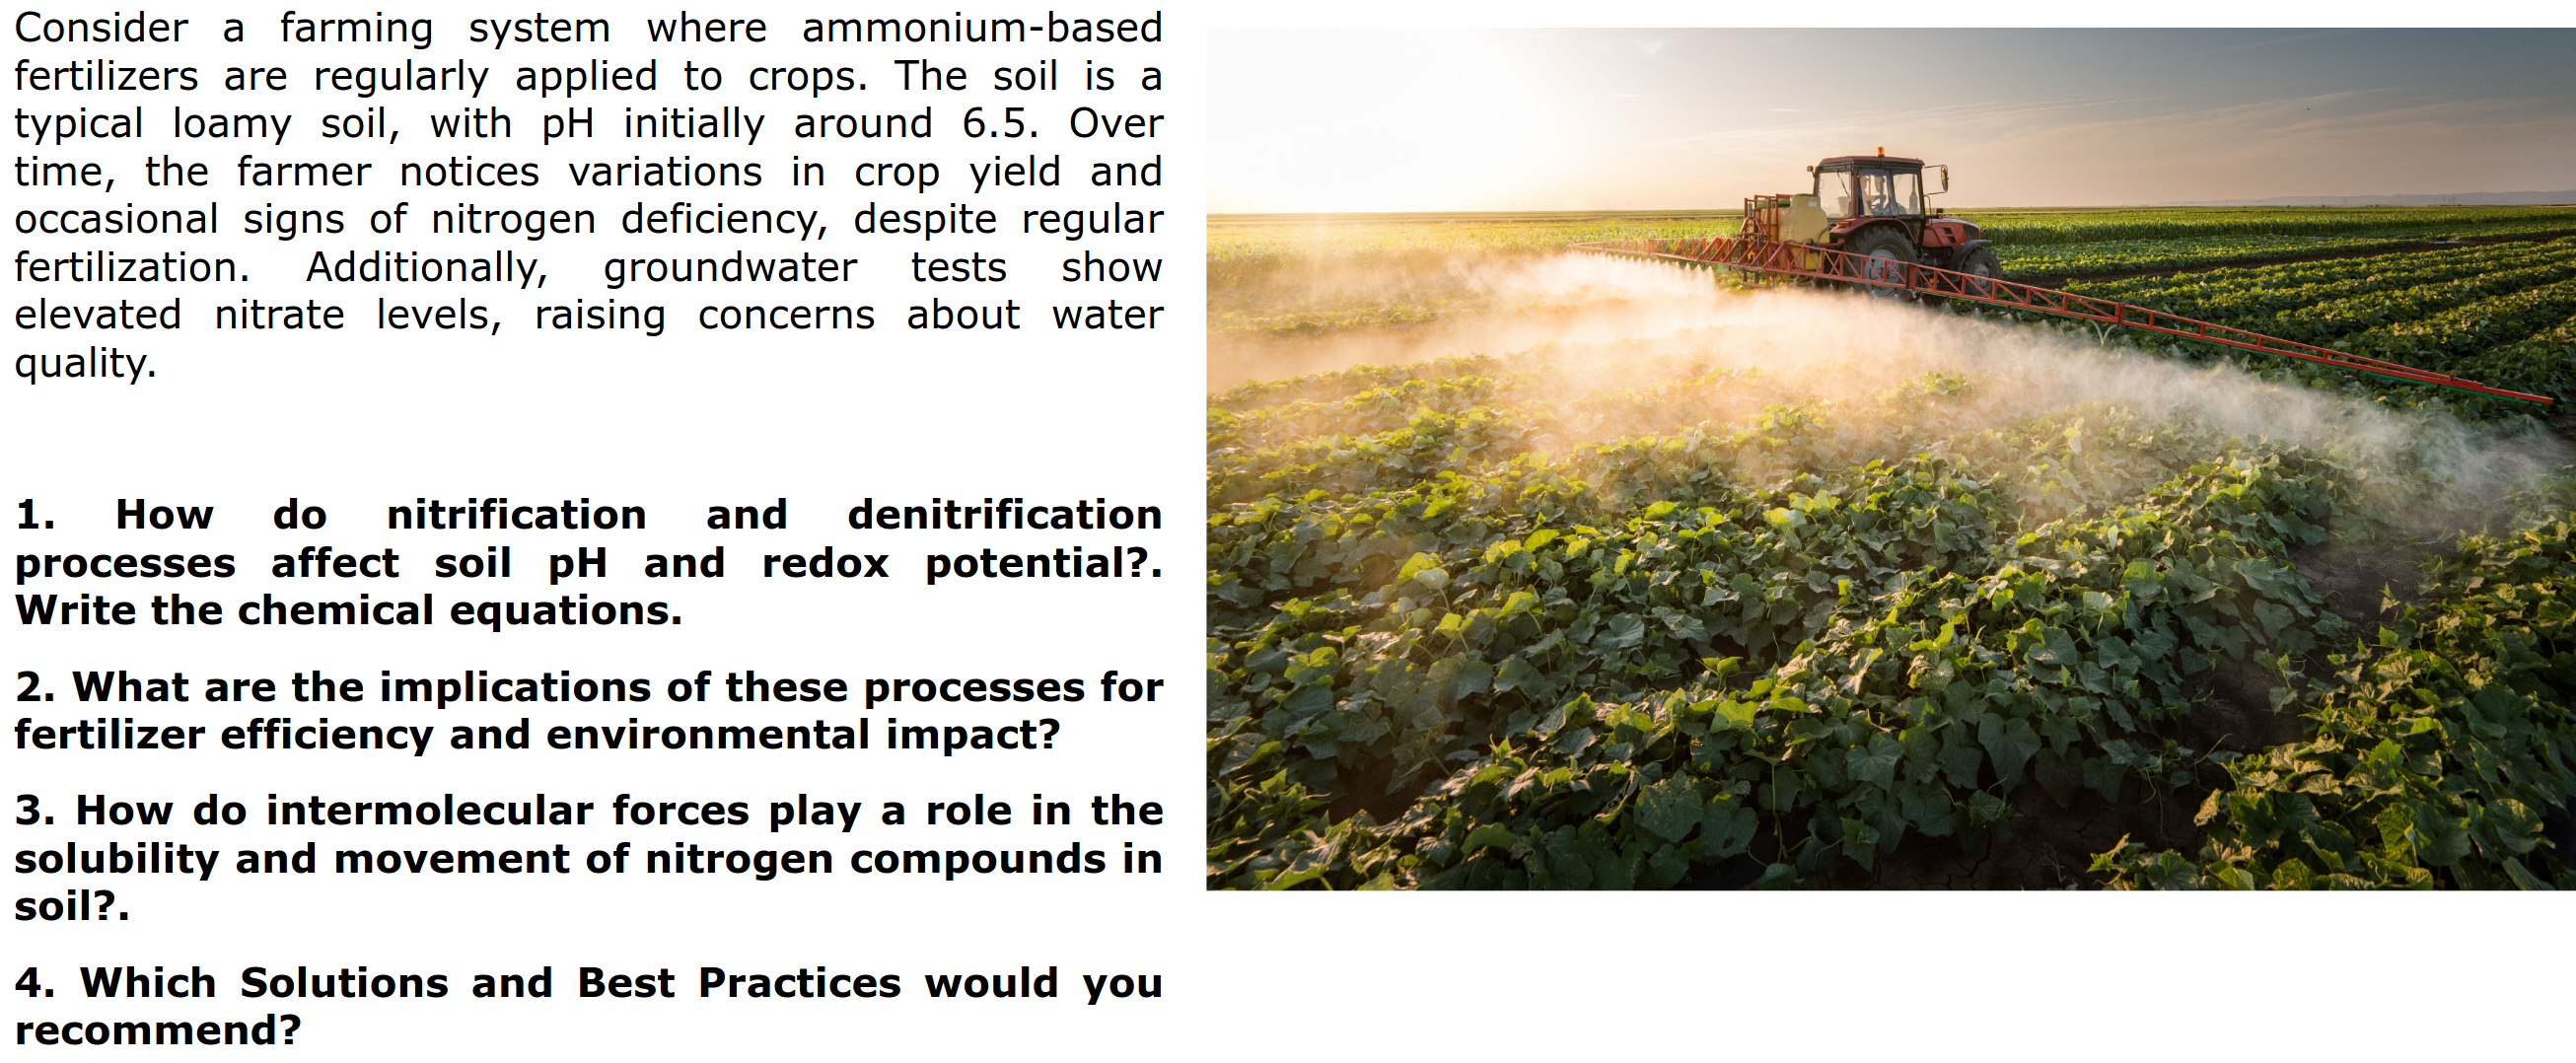
\includegraphics[width=\textwidth]{media1/SW04.png}

\subsection{Nitrification and denitrification}
\subsubsection{Nitrification}
The \textbf{nitrification process} converts ammonia (NH$_4$) into nitrite (NO$_2^-$) and finally
into nitrate (NO$_3^-$). This mechanism causes many hydrogenions to be released into the
soil, consequently increasing soil acidity and thus a decrease in pH.

The RedOx potential of soil decreases is inversely proportional to the increase in soil
oxidation. In an extremely oxidized environment, aerobic activity of bacteria is favored.

\textit{Ammonium to Nitrite}\\
\chemfig{2NH_{4}^{+} + 3O_{2}\ \to\ 2NO_{2}^{-} + 4H_{2}^{+} + 2H_{2}O}

\textit{Nitrite to Nitrate}\\
\chemfig{2NO_{2}^{-} +\; O_{2}\ \to\ 2NO_{3}^{-}}

\subsubsection{Denitrification}
The \textbf{denitrification process} reduces nitrate NO$_3^-$ first to nitrite NO$_2^-$ and then
converts it to nitrogen gas in the soil (N$_2$O) and then completes the cycle, releasing
it into the air as N$_2$.\\
The pH of the soil increases as a result of the reduction of the molecules, causing it to
return to more neutral conditions.

The RedOx potential is lowered during denitrification, because as the soil is reduced,
the anaerobic activity of bacteria in the soil is favored

\textit{Denitrification}\\
\chemfig{2NO_{3}^{-}\ \to\ N_{2} + 3O_{2}}

\newpage
\subsection{Fertilizer efficiency and environmental impact}
Due to the increase of acidity in the soil caused by the nitrogen reactions, the fertilizer
would then need to use a more basic solution to neutralize these effects and maintain a
balanced pH level. For environmental impact, since the crops require specific pH levels,
they may die or become tainted due to this change in acidity.

\subsection{Role of intermolecular forces}
Ammonium is a soluble compound meaning it can move easily in water whereas Nitrate is not
easily soluble meaning it could become "stuck" in the soil.

\subsection{Solutions and practices}
Our solutions where to either create a mixture in the fertilizer that is more basic to
neutralize the acidifying effects of nitrification/denitrification or to simply use less
fertilizer.






\end{document}
